\chapter{\IfLanguageName{dutch}{Stand van zaken}{State of the art}}
\label{ch:stand-van-zaken}

% Tip: Begin elk hoofdstuk met een paragraaf inleiding die beschrijft hoe
% dit hoofdstuk past binnen het geheel van de bachelorproef. Geef in het
% bijzonder aan wat de link is met het vorige en volgende hoofdstuk.

% Pas na deze inleidende paragraaf komt de eerste sectiehoofding.


In dit deel zal men toespitsen op de werking van een wayfinding applicatie, bij uitstek de concrete werking van het AI/AR mechanisme.

\section{Begrippen}
\subsection{AI (Artificiële intelligentie)}
Artificiële intelligentie of AI is een zeer groot fenomeen in de huidige IT-wereld. Men kan het beschrijven als intelligentie die wordt gedemonstreerd door machines. Op deze manier kunnen die apparaten de omgeving waarnemen en vervolgens acties ondernemen die het succesvol bereiken van een bepaald doel zal maximaliseren. In het algemeen staat de term AI ook gekend als de beschrijving van machines of computers die cognitieve acties uitvoeren die wij als mensen associeren met de menselijke geest. 

In deze bachelorproef wordt AI toegepast op het vlak van objectdetectie, het is de meest cruciale factor om een wayfinding applicatie te optimaliseren.
Objectdetectie zal in de wayfinding applicatie er voor zorgen dat de omgeving op een correcte manier wordt herkend, zo kan men een perfect beeld scheppen van welke objecten men afstand moet houden, bijvoorbeeld muren.

\subsubsection{Objectherkenning vs. Objectdetectie}
In Artificiële intelligentie heeft men twee verschillende manieren om objecten te identificeren, objectherkenning en objectdetectie. Het herkenningsproces is zeer gelijkaardig, maar toch zijn er zekere verschillen bij de uitvoering. Objectdetectie kan men beschouwen als een subset van objectherkenning, men zal de objecten herkennen op een simultane manier, maar bij objectdetectie wordt het object ook gelocaliseerd in de afbeelding. In de onderstaande afbeelding kan men het verschil duidelijk waarnemen, objectherkenning (links) en objectdetectie (rechts).

\begin{center}
	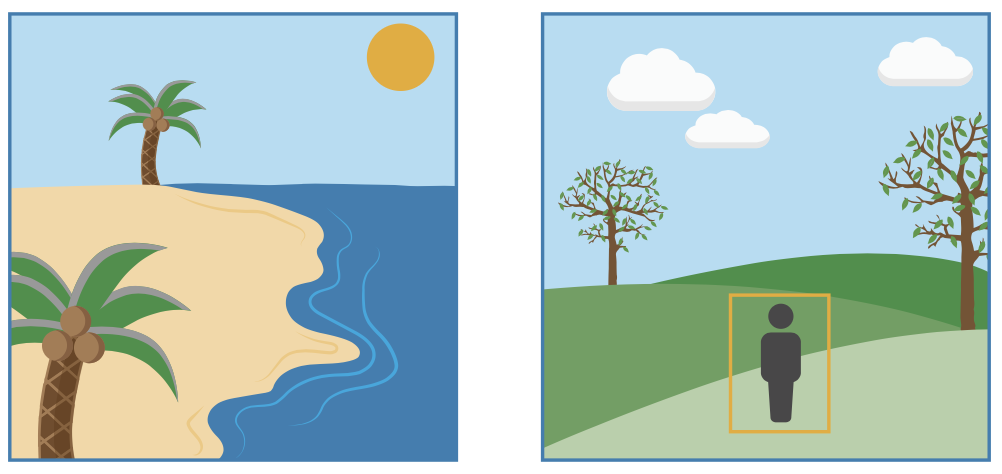
\includegraphics[scale=0.35]{objectdetectie.png}
\end{center}

\subsection{Werking van objectherkenning}
Om objectherkenning toe te passen kan je gebruik maken van twee verschillende manieren, namelijk 'Machine Learning' en 'Deep learning'. Beide technieken zullen objecten gaan herkennen, maar ze zijn verschillend op vlak van uitvoering.

\subsubsection{Machine learing}
Machine learning maakt gebruik van classificatie om een bepaald object te herkennen. Ten eerste zal men een trainingset opstellen, dit gebeurt door een verzameling van afbeeldingen samen te stellen en vervolgens de relevante punten aan te duiden. Het is zeer belangrijk om de juiste relevante punten aan te duiden, anders zal het systeem verkeerd getraind worden, waardoor men vervolgens een verkeerde output zal verkrijgen. Deze punten zullen er voor zorgen dat het systeem verschillende categorieën herkent. Vervolgens zal het leermodel deze informatie gebruiken om nieuwe objecten (objecten die nog niet gekend zijn in de trainingset) te analyseren en te classificeren.

\begin{center}
	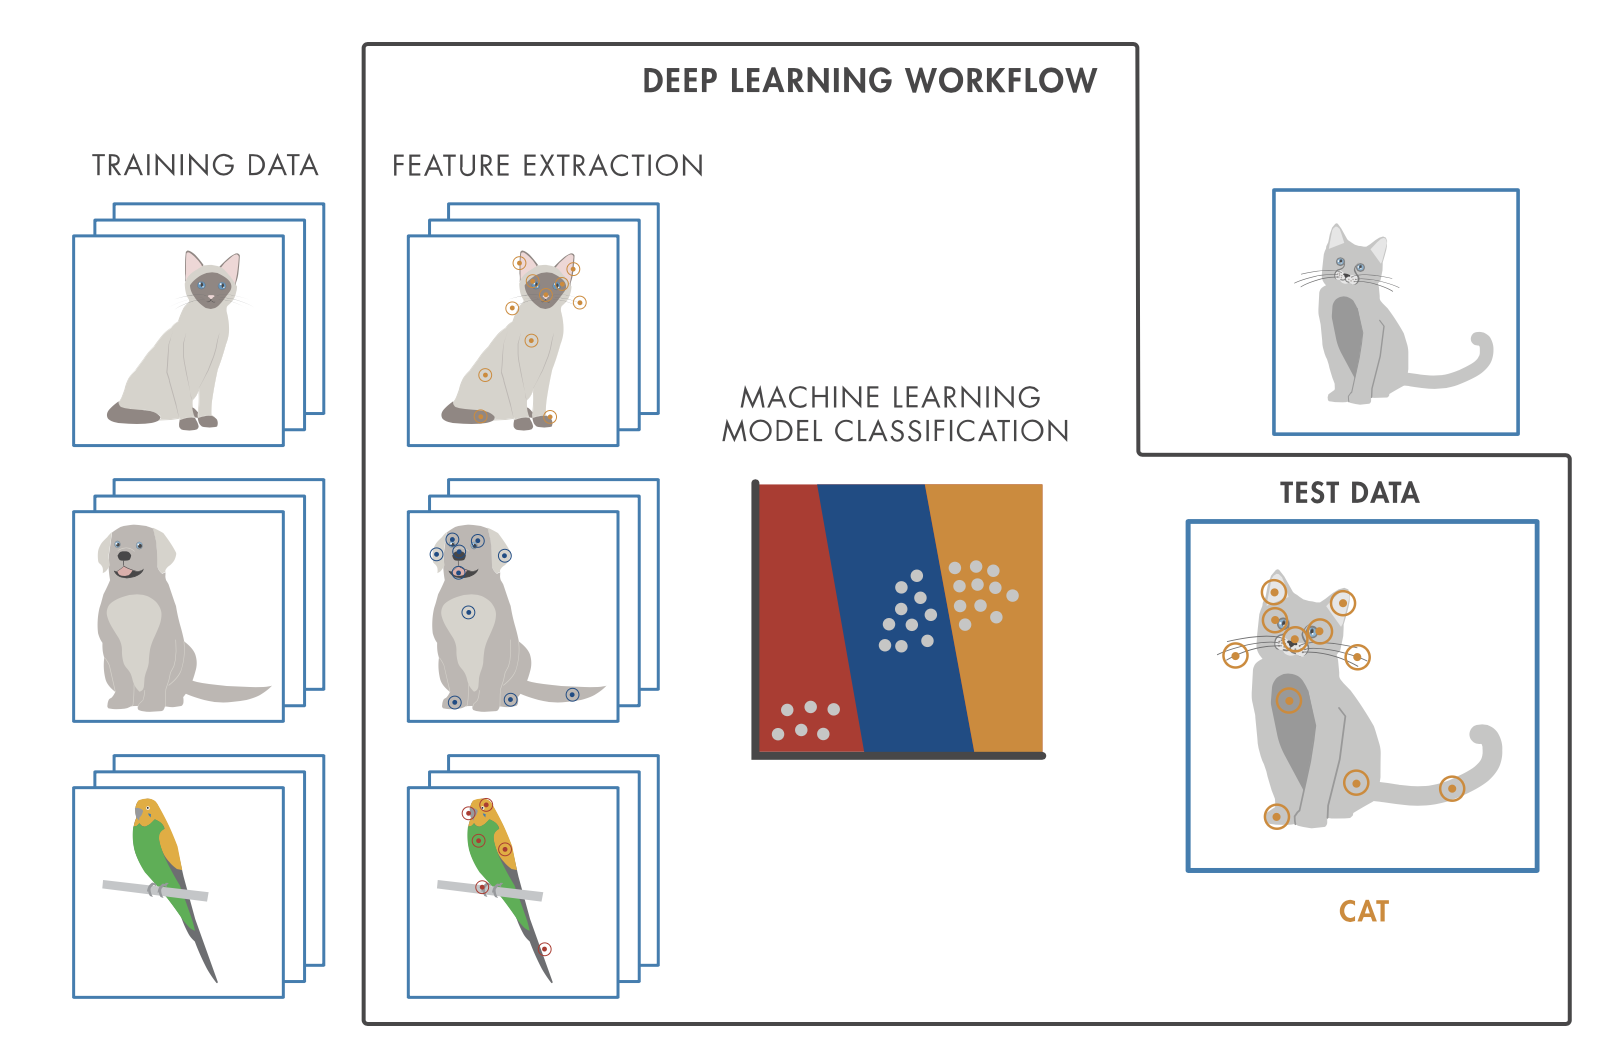
\includegraphics[scale=0.4]{machinelearning.png}
\end{center}

\subsubsection{Deep learning}
Deep learning maakt gebruik van convulationele neurale netwerken (CNN) om objecten te herkennen. Een CNN kan automatisch de aanhangende kenmerken van een object leren om dat object te identificeren, dit betekent dat een CNN bijvoorbeeld het verschil tussen auto's en vrachtwagens kan herkennen door middel van duizenden afbeeldingen te analyseren en vervolgens te leren welke kenmerken juist verschillend zijn.

\begin{center}
	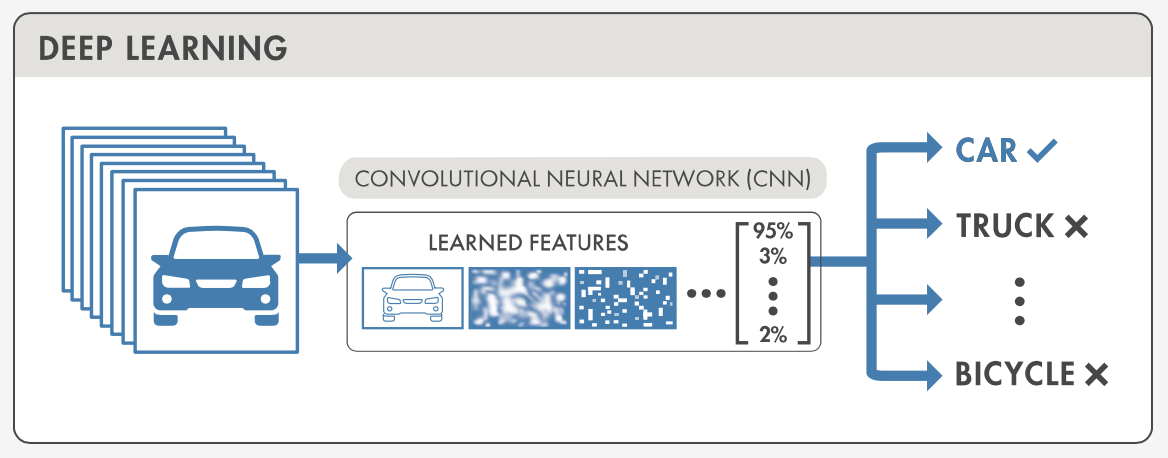
\includegraphics[scale=0.47]{deeplearning.png}
\end{center}

\subsection{AR (Augmented reality)}
Het concept AR is vandaag de dag niet meer uit het straatbeeld weg te denken, het wordt bijvoorbeeld gebruikt bij de Instagram -en Snapchat filters. Augmented reality of AR is een interactieve ervaring met de omgeving waarin objecten die zich in de echte wereld bevinden worden versterkt door computergegenereerde objecten. AR is iets wat al even bestaat, het werd bijvoorbeeld al gebruikt bij één van de eerste straaljagers, het visier van de piloot wordt in dit voorbeeld ondersteund door een computergegenereerd object dat de vijand zou moeten lokaliseren. Augmented reality werd pas populair bij de modale mens wanneer Naintic Pokemon Go lanceerde, het werd één van de meest gekende smarthonegames. In 2017 introduceerde Android en Apple, AR Core en AR Kit, het werd vervolgens voor developers veel eenvoudiger om AR-applicaties te creëren.

Het doel van Augemented reality in deze bachelorproef is om de route op een zo efficiënt mogelijke manier aan te geven, dit betekent dat er geen pijlen door objecten mogen gaan. Om een beeld te kunnen scheppen over het effectieve doeleinde, heeft men alvast een voorbeeldfoto toegevoegd.

\begin{center}
	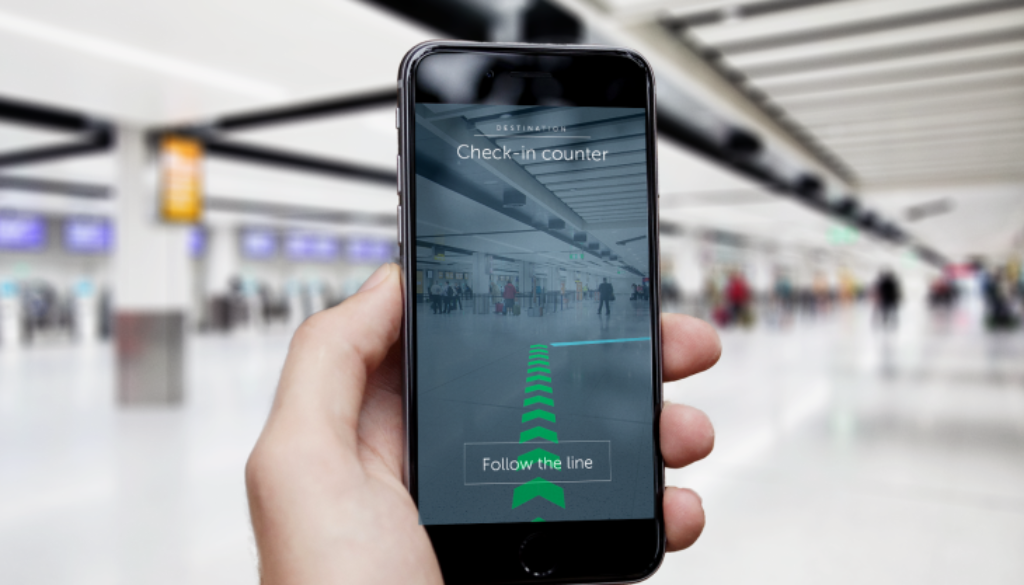
\includegraphics[scale=0.25]{wayfinding.png}
\end{center}

\subsection{Werking van Augmented realtiy}
Augmented reality kan momenteel op drie verschillende manieren worden uitgewerkt, namelijk door middel van SLAM, herkenning gebaseerd en locatie gebaseerd.

\subsubsection{SLAM (Simultaneous Localization and Mapping)}
Simultaneous Localization and Mapping of SLAM is de manier die het meest effectief en efficiënt werkt. SLAM lokaliseert sensoren ten opzichte van hun omgeving en brengt tegelijkertijd de omgeving in kaart, het is dus een zeer goede aanpak om complexe AR-simulatieproblemen op te lossen. Het SLAM-systeem is in feite een set van algoritmen die gericht zijn op het oplossen van gelijktijdige lokalisatie en het in kaart brengen van problemen. De meeste Augmented realitykits zijn reeds uitgerust met de mogelijkheid tot een SLAM-aanpak.

\subsubsection{Herkenning gebaseerd}
Herkenning gebaseerd gebruikt de camera van het gebruikte apparaat om bepaalde visuele markers of objecten te identificeren. Deze AR-technologie is bijgevolg zeer afhankelijk van de kwaliteit van de gebruikte camera, als deze de markers niet goed kan identificeren, dan zal het AR mechanisme niet goed werken.

Bij deze manier is het ook mogelijk om de positie en oriëntatie te berekenen. De markers op het scherm worden vervangen door een overeenkomstig 3D-object, dit maakt het mogelijk om het object meer in detail te bekijken door het bijvoorbeeld te roteren zodat men meerdere invalshoeken kan observeren.

\subsubsection{Locatie gebaseerd}
Locatie gebaseerd of 'markerless augmented reality' is een AR-technologie die alleen gebruikt maakt van een GPS, digitaal kompas, snelheidsmeter of versnellingsmeter om gegevens over de locatie te verzamelen, de augmented reality visualisaties worden met behulp van deze informatie geactiveerd. Een smartphone heeft genoeg sensoren om deze manier te kunnen realiseren. 

\subsection{AI + AR}
De samenhang van Artificiële intelligentie en Augmented reality is zeer cruciaal bij het optimaliseren van een wayfinding applicatie. Ten eerste is het belangrijk dat de objecten op een correcte manier worden herkend. Ten tweede is het zeer belangrijk dat de bevindingen van de objectherkenning op een correcte manier worden vertaald naar de AR omgeving. 

\section{Literatuurstudie}

In deze sectie zal men meer focussen op het onderzoek en de uitwerkingen die reeds werden gerealiseerd. Men zal deze algemene kennis kunnen gebruiken om mijn onderzoek te ondersteunen. Deze literatuurstudie staat ook in thema met de wayfinding-context, op deze manier is de verkregen informatie relevanter.

In het algemeen kan ik op voorhand al besluiten dat er reeds weinig onderzoek is gedaan naar de samenhang van 'Artificiële intelligentie' en 'Augemented reality' binnen de wayfinding-context. De termen AI en AR zijn afzondelijk van elkaar zeer gekend in de IT-wereld, men kan dit zelfs niet meer uit het straatbeeld wegdenken. Door de grote belangstelling voor AI en AR, en de minieme huidige onderzoekstoestand binnen de wayfinding-context wordt deze bachelorproef alleen maar interessanter.

\subsection{Artificiële intelligentie (AI)}

\subsubsection{Objectherkenning}
In het uitgave van ~\autocite{Liang2015}, \textcite{Liang2015} werd er onderzoek gedaan naar het gebruik van objectherkenning door middel van 'Convolutionele netwerken' of met andere woorden, 'Deep learning'. De auteurs werden geïnspireerd door 'Deep learning' omdat het reeds meerdere successen had geboekt bij andere computervisietaken. Omdat objectherkenning een zeer belangrijk factor is voor veel complexe systemen, wouden ze dit efficiënter maken en dus ook verbeteren, en dit door gebruik te maken van een geanvanceerde techniek, namelijk de convolutionele netwerken. 

Tijdens hun onderzoek werd het netwerk getest door middel van meerdere datasets, namelijk CIFAR-10, CIFAR-100, MNIST en SVHN. Deze datasets zijn zeer handig wanneer men convolutionele netwerken wilt testen, men hoeft dus geen data meer te verzamelen om te kunnen observeren of een netwerk wel degelijk goed functioneert. Het vinden van goede datasets is een cruciale factor bij het gebruik van AI, indien deze niet voldoen aan de eisen kan men ook geen bruikbare conclusies opstellen.

In het onderzoek verduidelijkt men ook nog eens het gebruik van 'Deep learning' zorgt voor betere resultaten. Het verhogen van de parameters in een CNN zorgde in het onderzoek voor nog een betere performantie, in tegenstelling met de 'gewone' feed-forward structuur. 

Uit de conclusie van hun onderzoek kan men besluiten dat een RCNN (recurrent convolutioneel netwerk) betere resultaten opleverd. Een recurrent convolutioneel netwerk is uitgebreider CNN, men gaat meer recurrente verbindingen (of parameters) toevoegen in elke laag. Deze structuur maakte het mogelijk om meer diepgang te creëren, men ging met andere woorden meer informatie verkrijgen uit elke laag, waardoor men meer kans kreeg op het juist eindresultaat. In de laatste fase van het onderzoek kon men andermaal besluiten dat het netwerk nog efficiënter werkte, bij het toevoegen van (nog) meer parameters.


Objectherkenning kan ook rechtstreeks gebruikt worden om de juiste weg te berekenen, dit wordt aangetoond in de studie van \autocite{Haikun2017}. In deze paper werd een wayfinding-ontwerp voor een virtuele wereld geoptimaliseerd. Vroeger werd een wayfinding-ontwerp handmatig opgesteld, hierbij moest men rekening houden met talloze verschillende parameters die mogelijks kunnen veranderen. Zo is het mogelijk dat de menselijke factoren als omgevingsfactoren  kunnen veranderen, een statisch ontwerp creëren die steeds voldoet aan relevante eisen is dus niet haalbaar.

Om dit probleem op te lossen werd 'Way to Go!' gecreërd, dit is een systeem dat automatisch een dynamisch wayfinding-ontwerp kan genereren voor verschillende navigatiemogelijkheden. Het systeem werkt als volgt. Ten eerste moet men een navigatiescenario specifiëren, met moet met andere woorden een route uitstippelen. Ten tweede zal het systeem automatisch een geoptimaliseerd wayfinding-ontwerp creëren met borden die op de juiste manier zijn geplaatst, rekening houdend met de zichtbaarheid van menselijke agenten en de mogelijkheid om fouten te maken tijdens een navigatie.  In het onderzoek evalueert men de resultaten door verschillende wayfinding-ontwerpen te vergelijken en laten zien dat het geoptimaliseerde wayfinding-ontwerp voetgangers effectief en efficiënt naar hun bestemming kan leiden. De aanpak kan de ontwerper van het ontwerp ook helpen om de bereikbaarheid van een bestemming vanaf verschillende locaties te visualiseren en eventuele "blinde" zones te corrigeren met extra bewegwijzering.

\subsubsection{Postionering}
 
\subsection{Augmented reality (AR)}

\subsubsection{Simultaneous Localization and Mapping (SLAM)}
Het onderzoek van \autocite{Zhang2017} heeft als hoofddoel om het leven voor slechtzienden makkelijk te maken. Men wenst dit doel te bereiken met behulp van een indoor wayfinding applicatie te creëren die deze bepaald groep mensen zal begeleiden bij het vinden van de weg, specifiek in gebouwen. Dit onderzoek is zeer vergelijkbaar met deze bachelorproef, het eindproduct kent bijna een grote gelijkenis, alleen wordt er in deze paper gebruik gemaakt van audio-ondersteuning. Men is er dan ook van overtuigt dat deze publicatie zal helpen bij het vinden van het gepaste eindresultaat.

In dit onderzoek probeert men huidige SLAM-technieken te verbeteren, volgens de state-of-the-art werden er steeds fouten bevonden bij het bepalen van de correcte positie, de zogekende 6-DOF-fout. De gekende aanpassingen die werden toegepast tijdens het onderzoek verbeterden niet alleen de 6-DOF-fout, maar ook de rekentijd. Dit resulteert in een snellere response naar de eindgebruiker, wat alleen maar een positieve invloed heeft op de gebruiksvriendelijkheid. In het onderzoek werden ook experimenten uitgevoerd, deze toonden daadwerkelijk aan dat de effectiviteit van het navigeren wel degelijk werd verbeterd voor slechtziende mensen.

\subsection{Artificiële intelligentie (AI) + Augmented reality (AR)}
Die paper van \autocite{Pouria2016} zal zeer veel hulp bieden, het eindresultaat van dit onderzoek kent namelijk een zeer grote overeenkomst met de objectieven van deze bachelorproef. Dit onderzoek gebruikt evenals hetzelfde soort toestel om te communiceren met de gebruiker.

In de uitwerking hield men rekening met de sensoren die men kan vinden in mobiele toestellen, hiermee ging men ook aan de slag. Deze sensoren hebben het mogelijk gemaakt om de locatie, koers en oriëntatie van de gebruiker te detecteren en om contextuele informatie uit verschillende bronnen van online gegevens te verkrijgen. Het combineren van de verkregen data van positionerings- en oriëntatiesensoren met camera's heeft het ook mogelijk gemaakt om praktische Augmented Reality (AR)-toepassingen op deze mobiele apparaten in te zetten. 

Voor de uitwerking van de paper werd een systeem gecreëerd dat een beeld geeft over de navigatiebeleving, dit werd gerealiseerd door middel van Augmented reality en continue feedback van de gebruiker ten opzichte van de dichtsbijzijnde oriëntatiepunten. Deze oriëntatiepunten zijn nodig voor de navigatie en om het juiste pad te vinden. De exacte positie werd bepaald door middel van GPS-sensoren, deze zijn reeds aanwezig in mobiele apparaten. Bovenop de GPS-data werd ook gebruik gemaakt van een beeldverwerkingsalgoritme die de juiste afstand berekent tot een oriëntatiepunt.Om de effectiviteit van het padvinden te verbeteren werd een machinaal leeralgoritme toegevoegd. Dit algoritme zal er voor zorgen dat men voor elke gebruiker een bewegingsprofiel kan opstellen, dit profiel zal er voor zorgen dat men steeds aanpassingen kan uitvoeren op de navigatie-instructies.

Uit de experimenten werd gebleken dat het gebruikte algoritme veel betere resultaten leverde als een 'normaal' turn-by-turn systeem, deze technologie wordt gebruikt bij de huidige GPS-toestellen.

